Zeigen Sie, dass die Funktion $f(x)=e^x/x$ keine elementare Stammfunktion
hat.

\begin{loesung}
Mit $\vartheta = e^x$ ist dies der polynomielle Fall für das Polynom
$p(\vartheta)= \frac1{x}\vartheta$.
Da eine exponentielle Erweiterung vorliegt, muss die
Risch-Differentialgleichung
\[
Dq_1 + Du q_1 = p_1
\quad\Rightarrow\quad
Dq_1 + q_1 = \frac{1}{x}
\]
durch eine rationale Funktion $q_1(x)$ gelöst werden.
Gäbe es eine Lösung $q_1(x)$, könnten wir diese
als gekürzten Bruch $q_1(x)=a(x)/b(x)$ schreiben, wobei
$b(x)$ normiert ist.
Wir erhalten dann nach Einsetzen und Multiplizieren mit $b(x)^2$
\begin{align*}
Da(x)\cdot b(x) - a(x) \cdot Db(x) + a(x) b(x) &= \frac{1}{x}b(x)^2.
\end{align*}
Alle Terme ausser dem zweiten sind offensichtlich durch $b(x)$ teilbar,
also muss auch $Db(x)$ durch $b(x)$ teilbar sein.
Da $Db(x)$ kleineren Grad als $b(x)$ hat, folgt $Db(x)=0$, $b(x)$ ist eine
Konstante $b(x)=b_0$.
Da $b(x)$ normiert ist, folgt ausserdem $b_0=1$.
Es bleibt daher
\begin{align*}
Da(x) + a(x) &= \frac{1}{x}.
\end{align*}
Auf der linken Seite steht ein Polynom, auf der rechten jedoch nicht.
Dieser Widerspruch zeigt, dass $q_1(x)$ in der verlangten Form nicht
existieren kann und daher die Stammfunktion nicht elementar ist.
\end{loesung}

%
% fig-ei.tex
%
% (c) 2026 Prof Dr Andreas Müller
%
\begin{figure}
\centering
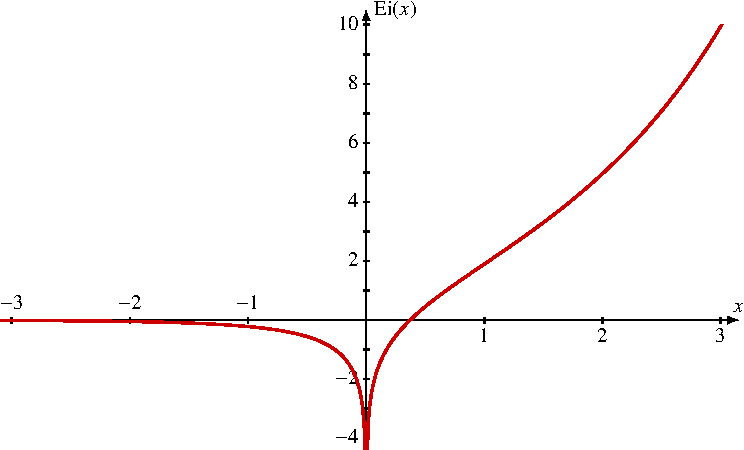
\includegraphics{chapters/070-intalg/images/ei.pdf}
\caption{Graph der Integralexponentialfunktion $\operatorname{Ei}(x)$.
\label{buch:intalg:604:ei}}
\end{figure}
%

\begin{diskussion}
Die Funktion
\begin{equation}
\operatorname{Ei}(x)
=
\int_{-\infty}^x \frac{e^t}{t}\,dt
\label{buch:intalg:risch:eqn:integralexponential}
\end{equation}
heisst die \emph{Integralexponentialfunktion}.
\index{Integralexponentialfunktion}%

Der Graph der Integralexponentialfunktion ist in
Abbildung~\ref{buch:intalg:604:ei} dargestellt.
$\operatorname{Ei}(x)$ ist nahe mit dem Integrallogarithmus
von Definition~\ref{buch:intalg:risch:def:integrallogarithmus}
verwandt, es gilt nämlich
\[
\operatorname{li}(x) = \operatorname{Ei}(\log x)
\qquad\Leftrightarrow\qquad
\operatorname{li}(e^x) = \operatorname{Ei}(x).
\]
Wie beim Integrallogarithmus muss die Singularität des Integranden in
\eqref{buch:intalg:risch:eqn:integralexponential}
bei $t=0$ mit dem Hauptwert überbrückt werden.
\end{diskussion}
